%!TEX root = irma-crypto.tex

\usetheme[progressbar=frametitle,block=fill]{metropolis}

\useoutertheme{metropolis}
\useinnertheme{metropolis}
\usefonttheme{metropolis}

\usepackage{outlines}
\usepackage{appendixnumberbeamer}
\usepackage{array}
\usepackage{booktabs}

\usepackage{xspace} 
\newcommand{\themename}{\textbf{\textsc{metropolis}}\xspace}

\usepackage{tikz}
\usepackage{amsmath}
\usepackage{mathtools}
\usepackage{wrapfig}
\usepackage{makecell}
\usepackage[makeroom]{cancel}
\usepackage{xcolor}
\usepackage{calc}
\usepackage{pgfpages}

\def\XLR#1{\xleftrightarrow[\rule{1.5cm}{0pt}]{#1}}% \rule defines the width
\def\XR#1{\xrightarrow[\rule{1.5cm}{0pt}]{#1}}
\def\XL#1{\xleftarrow[\rule{1.5cm}{0pt}]{#1}}

\setbeamertemplate{note page}[plain]

\makeatletter
\newif\ifOnBeamerModeTransition
\newcommand{\slideselection}{1-}%
\newenvironment{handoutframeselect}[1][1-]{%
  \begingroup%
  \mode<handout>{%
    \gdef\beamer@currentmode{beamer}%
    \OnBeamerModeTransitiontrue%
    \renewcommand{\slideselection}{#1}}%
}{%
  \ifOnBeamerModeTransition%
    \OnBeamerModeTransitionfalse%
    \gdef\beamer@currentmode{handout}%
  \fi%
  \endgroup%
}
\makeatother

%Logo
\AtBeginEnvironment{minted}{\renewcommand{\fcolorbox}[4][]{#4}}
\AtBeginSection[]{\begin{frame}<beamer>\frametitle{Topic}\tableofcontents[currentsection]\end{frame}}
\LetLtxMacro{\OldIncludegraphics}{\includegraphics}
\renewcommand{\includegraphics}[2][]{\OldIncludegraphics[height=0.8\textheight,keepaspectratio, #1]{#2}}

\usepackage{textpos}
\addtobeamertemplate{frametitle}{}{%
\begin{textblock*}{100mm}(.99\textwidth,-0.9cm)

\includegraphics[height=0.75cm]{assets/logo.png}
\end{textblock*}}

\addtobeamertemplate{title}{}{%
\begin{textblock*}{100mm}(.99\textwidth,-3cm)

\includegraphics[height=0.75cm]{assets/logo.png}
\end{textblock*}}

\title{IRMA's Idemix core}
\subtitle{Understanding the crypto behind selective, unlinkable attribute disclosure}
\date{July 24, 2022}
\author{Maja Reißner \texorpdfstring{\\}{,} Sietse Ringers}
\institute{}
\setbeamertemplate{frame footer}{\insertshorttitle}

% STYLE
\makeatletter
\setlength{\metropolis@titleseparator@linewidth}{2pt}
\setlength{\metropolis@progressonsectionpage@linewidth}{1pt}
\setlength{\metropolis@progressinheadfoot@linewidth}{1pt}
\makeatother

\definecolor{darkblue}{HTML}{074487}
\definecolor{lightblue}{HTML}{1db2e4}
\definecolor{pdBlue}{HTML}{1485bc}
\definecolor{pdGreen}{HTML}{4ab19d}
\definecolor{pdNeonGreen}{HTML}{a2ce4e}
\definecolor{dark}{HTML}{24373b}

%Setting colors
\setbeamercolor{alerted text}{fg=pdBlue}
\setbeamercolor*{palette primary}{fg=dark,bg=gray!15!white}
\setbeamercolor{progress bar}{fg=pdBlue}
\setbeamercolor{example text}{fg=pdGreen}
\setbeamercolor{background canvas}{bg=white}

\setbeamertemplate{frame footer}{}

\begin{document}

\def\titlepage{
  \usebeamertemplate{title page}% just to get rid of the maketitle warning
}
\maketitle

\begin{frame}{Flip and Flap}
  \begin{center}
    \begin{tabular}{rl}
      \parbox{0.4\textwidth}{
        \begin{center}
          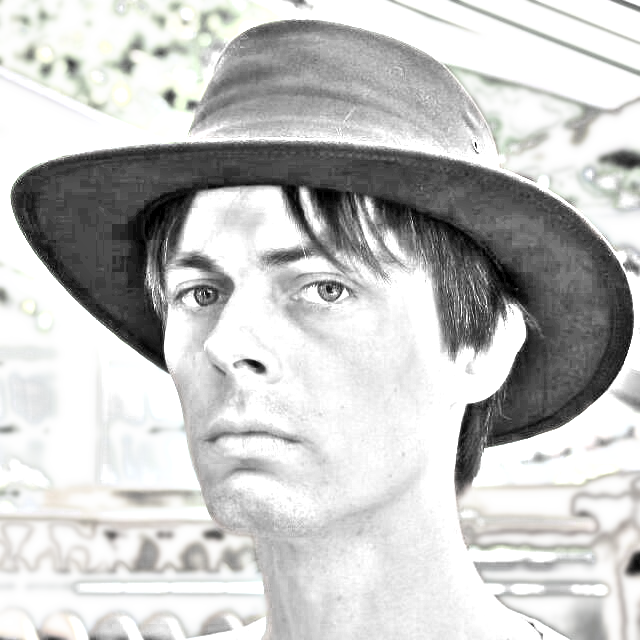
\includegraphics[width=40mm]{Pictures/flipFin.png}\\
          Sietse Ringers
        \end{center}
      }
      &
      \parbox{0.4\textwidth}{
        \begin{center}
          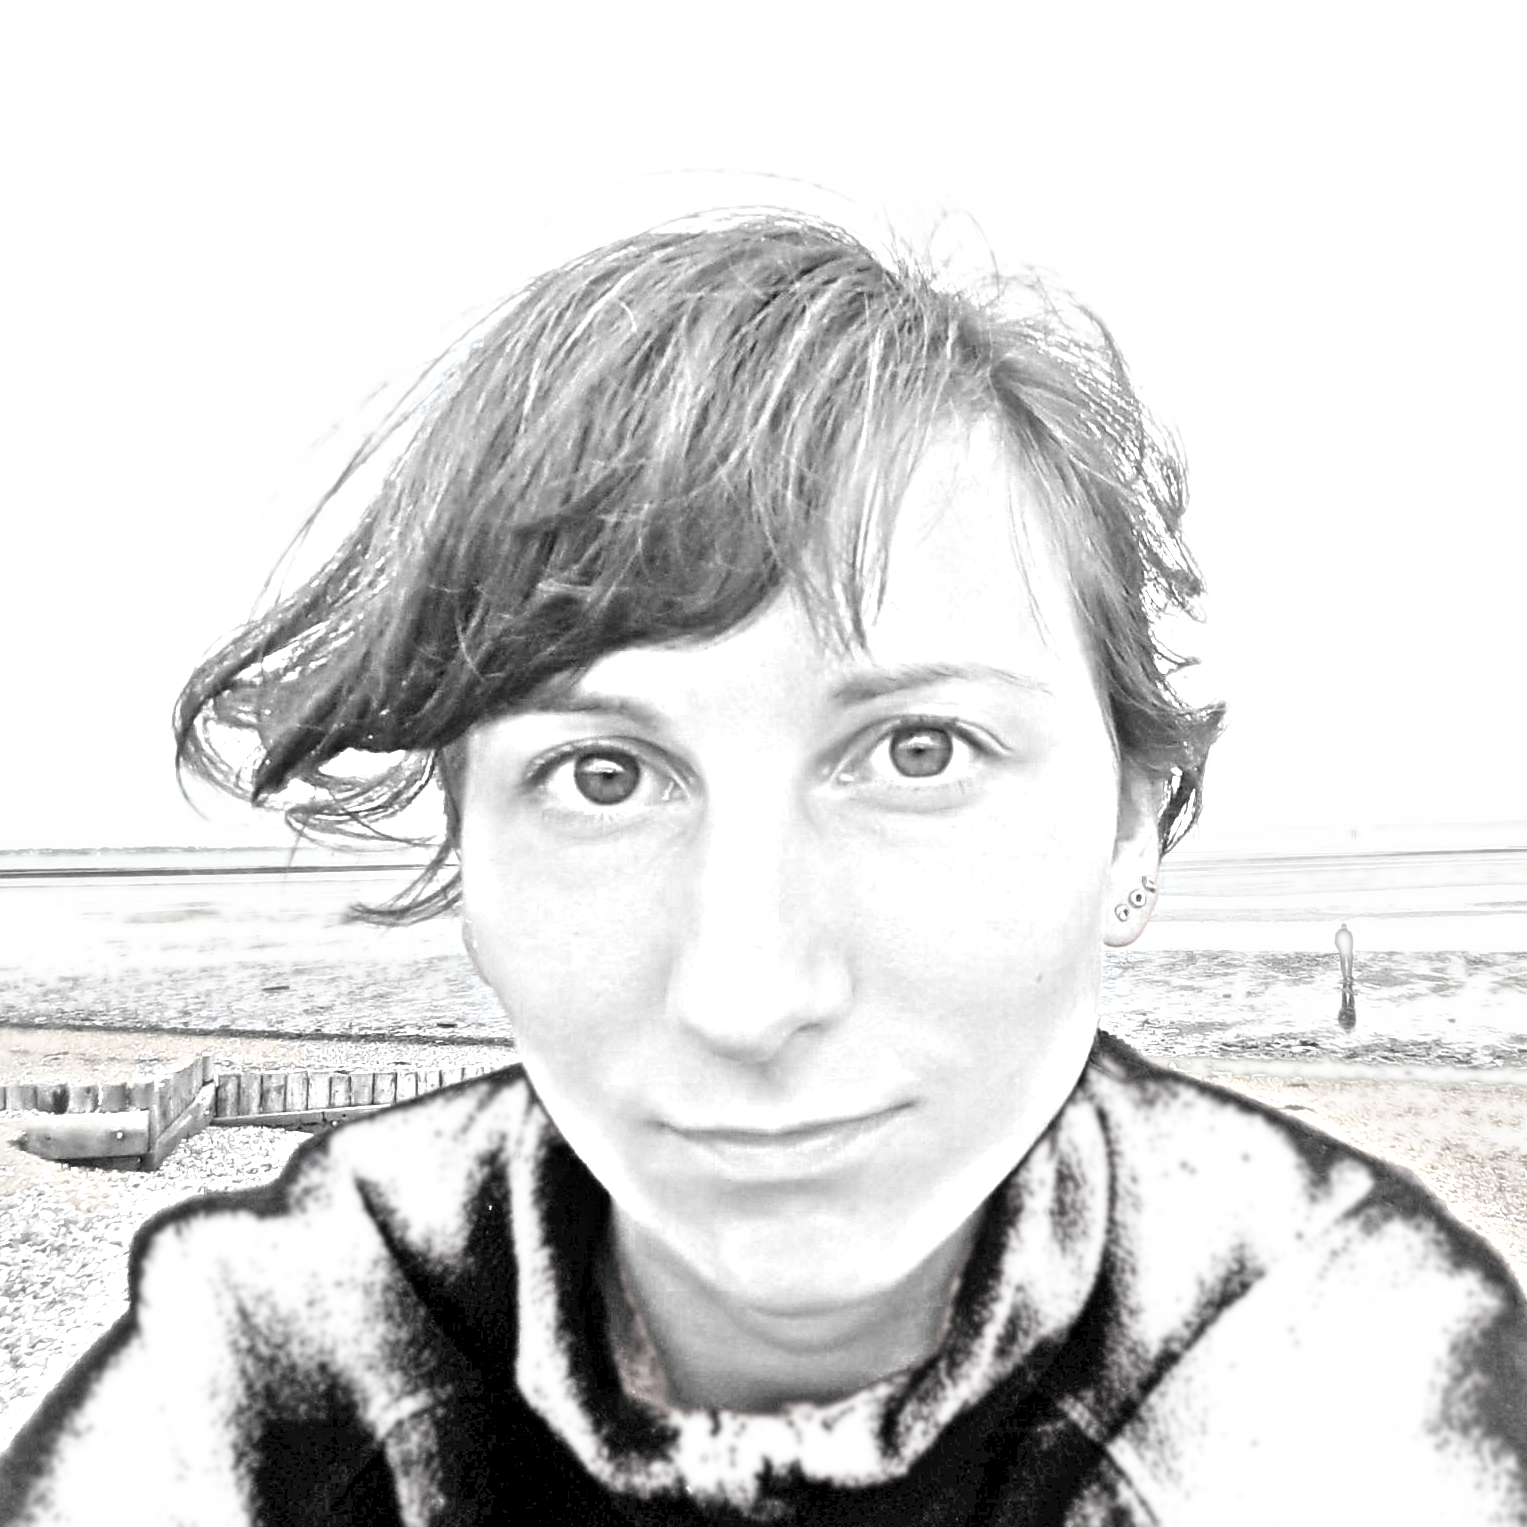
\includegraphics[width=40mm]{Pictures/flapFin.png}\\
          Maja Reißner
        \end{center}
      }
    \end{tabular}
  \end{center}
  \note{
    \begin{outline}
      \1 Maja Reißner, developer, 1.5 years
      \1 Sietse Ringers, architect, 6 years
      \1 At SIDN, previously Privacy by Design Foundation
      \1 Prerequisites:
        \2 IRMA app
        \2 basic familiarity with crypto
    \end{outline}
  }
\end{frame}

\begin{frame}{Introduction}
  \centering
  Self-Sovereign Identity \\[2em]
  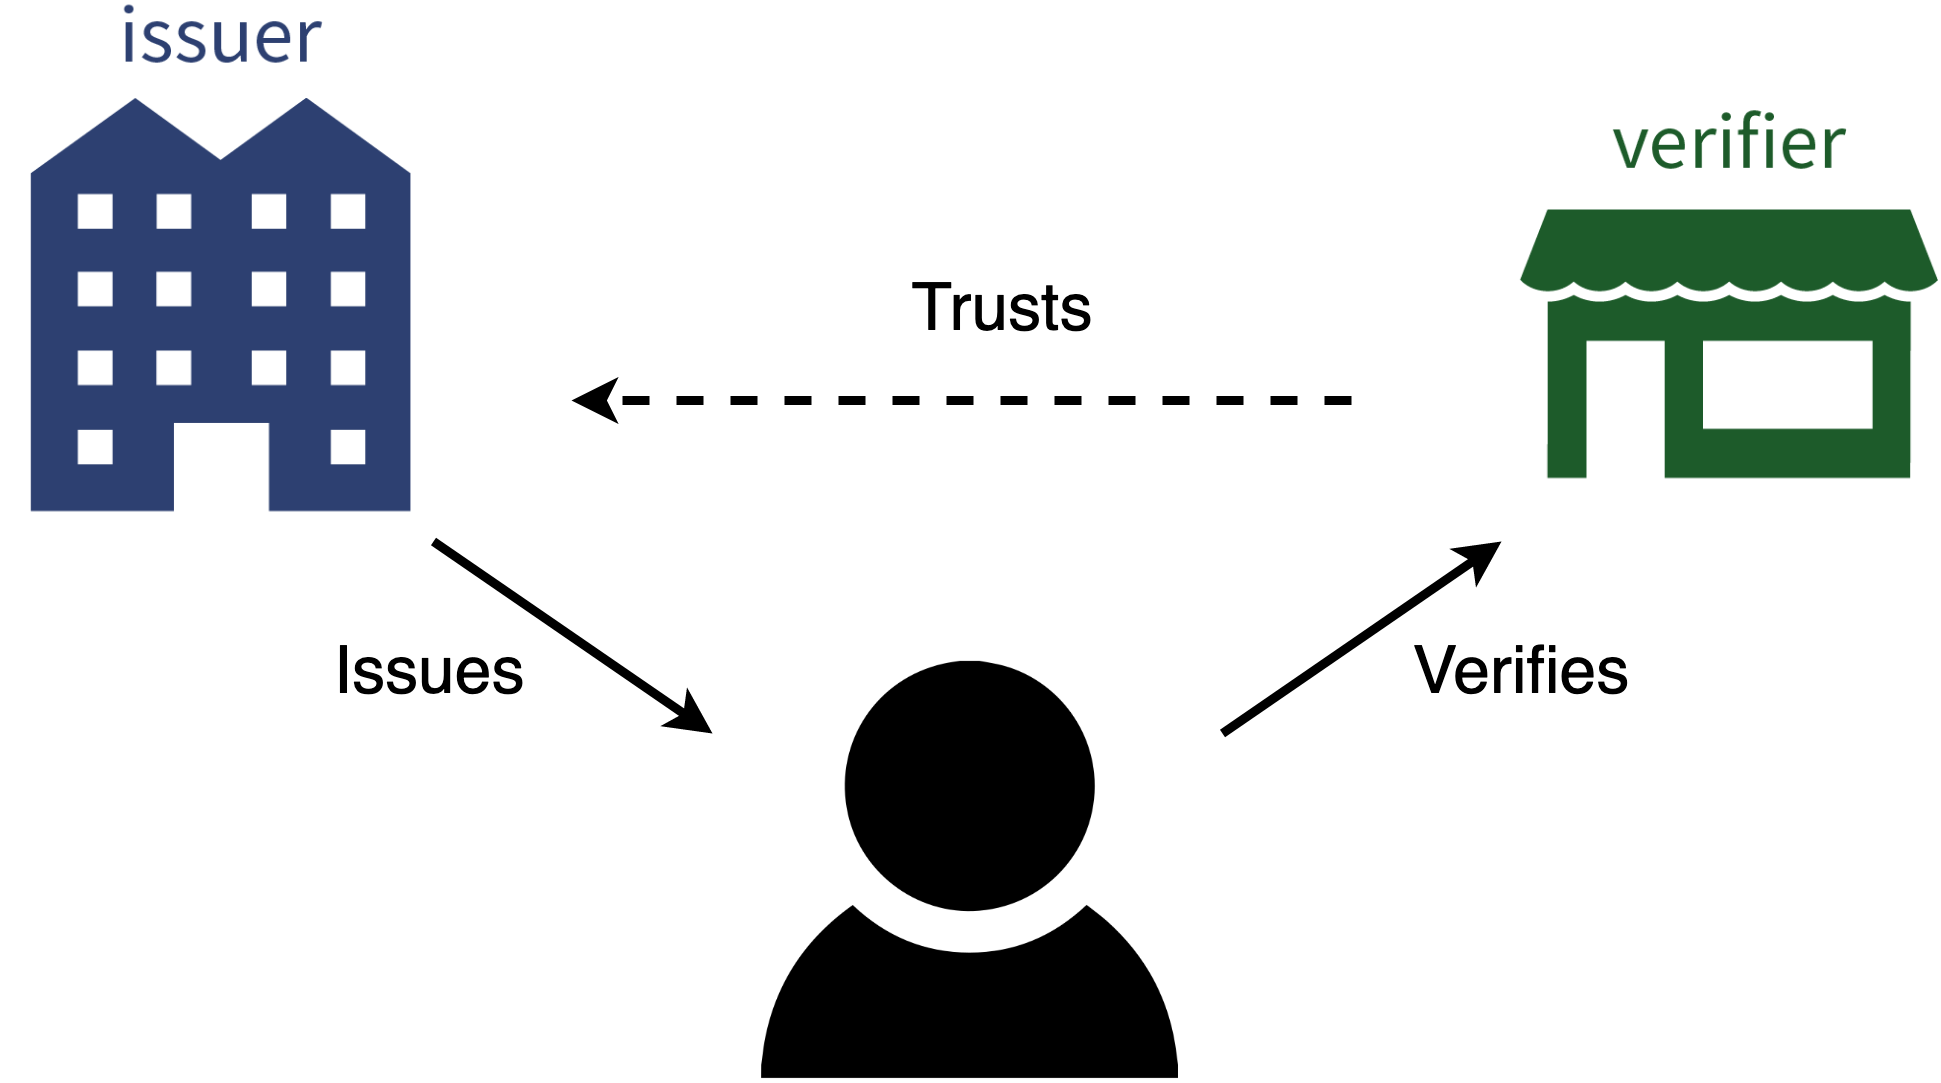
\includegraphics[width=9cm]{Pictures/SSI-diagram.png}
  % Plaatje gemaakt op https://app.diagrams.net, source SSI-diagram.drawio
  \note{
    \begin{itemize}
      \item IRMA is an Idemix implementation
      \item Names, concepts:
        \begin{itemize}
          \item disclosure
          \item holder
          \item verifier
          \item issuer
        \end{itemize}
      \item We focus on disclosure
    \end{itemize}
  }
\end{frame}

\begin{frame}{Introduction}
  \centering The offline world, using a paper diploma: \\~\\~\\
  \begin{columns}[c,onlytextwidth]
    \column{0.45\textwidth}
    \begin{minipage}[t][3cm][t]{4.5cm}
      \only<1>{\begin{block}{Diploma}
        \vspace{0.5em}
          \textbf{Sietse Ringers}, \\
          born on \textbf{July, 11th 1984}, \\
          has earned a \textbf{PhD} at \\
          \textbf{University of Groningen}.
          \vspace{0.5em}
        \end{block}
        \begin{tikzpicture}[very thick,overlay, remember picture]
          \draw[fill=red, thick, opacity=0.4] (4.5,0.5) circle (0.6cm) node {sign};
        \end{tikzpicture}
      }
      \only<2-3>{\begin{block}{Diploma}
        \vspace{0.5em}
          \textbf{xxxxxxxxxxx},\phantom{S} \\
          born on \textbf{xxxxxxxxxxx},\phantom{J} \\
          has earned a \textbf{PhD} at \\
          \textbf{xxxxxxxxxxx}.\phantom{Jy}
          \vspace{0.5em}
        \end{block}
        \begin{tikzpicture}[very thick,overlay, remember picture]
          \draw[fill=red, thick, opacity=0.4] (4.5,0.5) circle (0.6cm) node {sign};
        \end{tikzpicture}
      }
      \only<4->{\begin{block}{Diploma}
        \vspace{0.5em}
          \textbf{zzzzzzzzzzz},\phantom{S} \\
          born on \textbf{zzzzzzzzzzz},\phantom{J} \\
          has earned a \textbf{PhD} at \\
          \textbf{zzzzzzzzzzz}.\phantom{Jy}
          \vspace{0.5em}
        \end{block}
        \begin{tikzpicture}[very thick,overlay, remember picture]
          \draw[fill=red, thick, opacity=0.4] (4.5,0.5) circle (0.6cm) node {sign};
        \end{tikzpicture}
      }
    \end{minipage}
    \column{0.6\textwidth}
    \begin{itemize}
      \item<2-> \emph{Feature:} Selective disclosure
      \item<3-> \emph{Problem:} Replay attacks
      \item<4-> \emph{Feature:} Unlinkability
    \end{itemize}
  \end{columns}
  \note{
    \begin{outline}
      \1 Let's see how authentication works offline
      \1 Use case: I want to apply for a job on a website, using my diploma
        \2 Used throughout. See the box
        \2 Bold stuff = attributes
      \1 Features:
        \2 Show diploma as is
        \2 Discrimination against nationality, age, etc $\Rightarrow$ selective disclosure
        \2 unlinkability: suppose I want to apply to two jobs at one employer
    \end{outline}
  }
\end{frame}
% TODO: definities sig scheme / cred scheme

\begin{frame}{Contents of this talk}  
  \begin{columns}[T,onlytextwidth]
    \column{0.55\textwidth}
     \vspace{1em}
      Goal is to understand:\\
      \vspace{1em}
      \href{https://github.com/privacybydesign/gabi/blob/d1eff7721dcad9cef411b340c67945da32ca2979/clsignature.go}{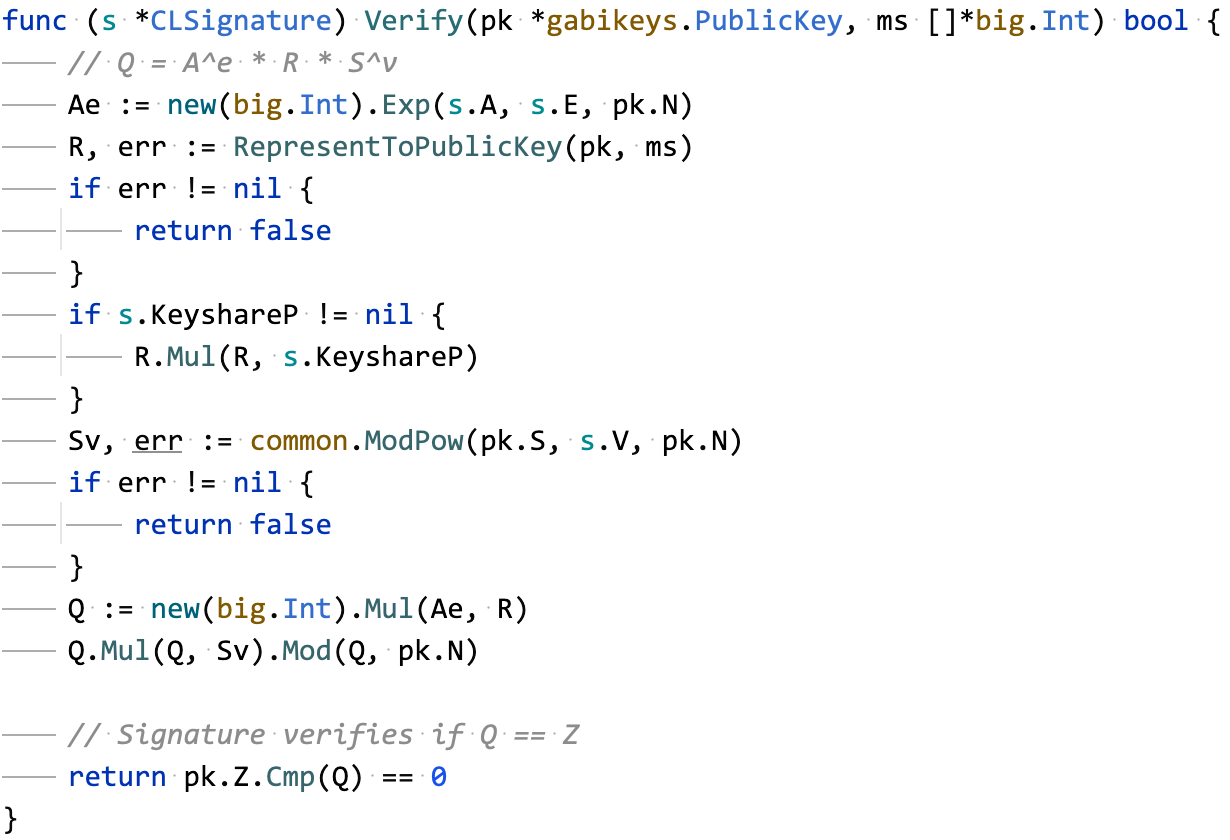
\includegraphics[width=8cm]{Pictures/CLSignatureVerifySnippet.png}}
    \column{0.05\textwidth}
    \column{0.4\textwidth}
      \vspace{2em}
      \uncover<2->{
      $$ \tilde{A}^e = \frac{Z}{S^{\tilde{v}} \displaystyle \prod_{i=0}^{k} R_i^{a_i}} \bmod n $$
      }
      \vspace{0.5em}
      \uncover<3->{
        \begin{outline}
        \1 Selective disclosure
        \2 Distinguish attributes
        \2 Hide attributes
        \1 Ownership of the credential
        \1 Unlinkability
        \1 Disclosure of multiple credentials
        \end{outline}
      }
    \end{columns}
  \note{
    Code fragment is from gabi, see GitHub
  }
\end{frame}

\begin{frame}{Distinguishing attributes}
  \begin{columns}[onlytextwidth]
    \column{0.7\textwidth}
    \\~\\
    Textbook RSA:\\
    $$A = M^d  \bmod n$$\\
    Verify with: $$A^e = M \bmod n$$\\
    \uncover<2->{
    \vspace{0.5em}
    Signature scheme which differentiates attributes:
    $$M= \frac{Z}{S^v R_1^{a_1}R_2^{a_2}}$$
    }
    \uncover<3->{
      \boldmath$$A^e= \frac{Z}{S^v R_1^{a_1}R_2^{a_2}} \bmod n$$\\
      \unboldmath
    }
    \uncover<4->{
    \vspace{1.5em}
    $\rightarrow$ \textbf{Camenisch-Lysyanskaya signature scheme}
    }
    \column{0.3\textwidth}
    \begin{minipage}[t][3cm][t]{4cm}
      \begin{block}{Diploma}
        \vspace{0.5em}
          Sietse Ringers \\
          has earned a PhD.
          \vspace{0.5em}
        \end{block}
        \begin{tikzpicture}[very thick,overlay, remember picture]
          \draw[fill=red, thick, opacity=0.4] (4,0.5) circle (0.6cm) node {sign};
        \end{tikzpicture}
    \end{minipage}
    \hspace{1em}

    \uncover<2->{
      \begin{minipage}[t][3cm][t]{4cm}
        \begin{block}{Diploma}
          \vspace{0.5em}
          name: \textbf{Sietse Ringers}, \\
          title: \textbf{PhD}
          \vspace{0.5em}
        \end{block}
        \begin{tikzpicture}[very thick,overlay, remember picture]
          \draw[red, thick] (4,0.5) circle (0.6cm) node {$A, e, v$};
        \end{tikzpicture}
      \end{minipage}
    }
  \end{columns}
  \note{
    Overview:
    \begin{itemize}
      \item digital signature
      \item cannot hide data as signature would not validate
      \item need signature scheme that distinguishes attributes
    \end{itemize}
    \vspace{1em}
    M fine-grained:
    \begin{itemize}
      \item attribute represented by a
      \item R as constants
      \item Z, S also part of public key
    \end{itemize}
    \vspace{1em}
    About CL:
    \begin{itemize}
      \item signature scheme called Camenisch-Lysyanskaya
      \item verification equation like RSA
      \item e part of signature, v explained later
    \end{itemize}
    % TODO?
    % issuer initially generates modulus n similar to RSA
    % issuer generates constants Z, S and bases R for as many attributes as needed
    % issuer publishes n, Z, S, R's
    % each attribute type gets its own fixed R
    
    % mention Z for unforgeability, not detailed, just mention
    % when signing during issuance, v is chosen randomly
  }
\end{frame}

\begin{frame}{Camenisch-Lysyanskaya (CL) signature scheme}
  \begin{columns}[onlytextwidth]
    \column{0.6\textwidth}
    \\~\\
    \textbf{Issuer setup}\\
    Choose private key $p,q$ so that $n = pq$\\
    Choose constants $Z, S, R_1,...,R_i$\\
    Share public key $(Z, S, R_1,...,R_i, n)$\\[1em]
    \textbf{During issuance of a credential}\\
    Choose $e, v$\\
    Calculate\\
    $$A= \left(\frac{Z}{S^v R_1^{a_1}R_2^{a_2}}\right)^{e^{-1}} \bmod n$$\\[1em]
    Share signature $(A,e,v)$\\[1em]
    \column{0.4\textwidth}
    \textbf{Verification equation}\\
      \boldmath$$A^e= \frac{Z}{S^v R_1^{a_1}R_2^{a_2}} \bmod n$$\\
      \unboldmath
      \vspace{5em}
  \end{columns}
  \note{
    About CL:
    \begin{itemize}
      \item signature scheme called Camenisch-Lysyanskaya, CL
      \item setup pq similar to RSA, public key (Z,S,R's,n)
      \item during issuance e,v; calculate A
      \item results in (A,e,v)
      \item we'll focus on verification equation
      \item capital numbers from public key
    \end{itemize}
  }
\end{frame}

\begin{frame}{Hiding an attribute}
  \vspace{2em}
  \begin{columns}[onlytextwidth]
    \column{0.7\textwidth}
  Signature verification:\\
  $$ A^e = \frac{Z}{S^v \only<1>{R_1^{a_1}}\only<2->{H}R_2^{a_2}} $$\\
  $$ H = R_1^{a_1}$$
  \\~\\~\\
\column{0.3\textwidth}
  \begin{minipage}[t][3cm][t]{4cm}
    \begin{block}{Diploma}
      \vspace{0.5em}
      name: \textbf{xxxxxxxx}, \\
      title: \textbf{PhD}
      \vspace{0.5em}
    \end{block}
    \begin{tikzpicture}[very thick,overlay, remember picture]
      \draw[red, thick] (4,0.5) circle (0.6cm) node {$A, e, v$};
    \end{tikzpicture}
  \end{minipage}
\end{columns}
  \only<2>{
  \vspace{0.5em}
  \begin{columns}[onlytextwidth]
    \column{0.5\textwidth}
      \textbf{Problem:} Forgery of other attributes.\\
      \vspace{1em}
      New example, given:\\
      $a_1$ ... name (to be hidden)\\
      $a_2$ ... age = 17
      \vspace{1em}
      \column{0.5\textwidth}
      Then I could forge my age to 18, like this:
      \\~\\
      claim $a_2 = 18$; \hspace{1em} $H' = HR_2^{-1}$
      $$ A^e = \frac{Z}{S^v {\color{red}H'}R_2^{a_2}} = \frac{Z}{S^v ({\color{red}H\cdot R_2^{-1}})R_2^{a_2}}= \frac{Z}{S^v H R_2^{{\color{red}a_2 - 1}}} $$
  \end{columns}
  }
  \uncover<3->{\textbf{Schnorr's Zero Knowledge (ZK)} protocol, given $H=R^a$\\
  \begin{center}
    \begin{tabular}{rcl@{\hskip 1.5cm}l}
      choose random $t$ &&&\\
      $U = R^t \bmod n$ & $\xrightarrow{\quad U\quad}$&&\textbf{commitment}\\
      &$\xleftarrow{\quad c\quad}$ & choose random $c$ &\textbf{challenge} \\
      $r = t + ca$ & $\xrightarrow{\quad r\quad}$ & $R^rH^{-c} \stackrel{?}{=} U \bmod n$ &\textbf{response}
    \end{tabular}}
  \end{center}
  \note{
    Hide name:
    \begin{itemize}
      \item replace $R^a$ by H
      \item hides a, infeasible for discrete log problem
      \item IF signature scheme is just share A,e,v,a2 and H THEN forgery possible
    \end{itemize}
    \vspace{1em}
    Problem: forgery of other attributes
    \begin{itemize}
      \item example with age since it's a number already
      \item need to proof knowledge of the attribute value
    \end{itemize}
    \vspace{1em}
    Schnorr protocol
    \begin{itemize}
      \item 3-step protocol
      \item proof in ZK
      \item indeces skipped
      \item t much bigger than ca, so t masks the attribute
    \end{itemize}
  }
\end{frame}

\begin{frame}{Proof why Schnorr's Zero Knowledge protocol works}
  \begin{center}
    \vspace{0.5em}
    \begin{tabular}{rll@{\hskip 1.5cm}l}
      given $H=R^{a}$ &&&\\
      choose random $t$ &&&\\
      $U = R^t \bmod n$ & $\xrightarrow{\quad U\quad}$&&\textbf{commitment}\\
      &$\xleftarrow{\quad c\quad}$ & choose random $c$ &\textbf{challenge} \\
      $r = t + ca$ & $\xrightarrow{\quad r\quad}$ & $R^rH^{-c} \color{red}\stackrel{?}{=}\color{black} U  \bmod n$ &\textbf{response}\\
      \vspace{0.2em}\\
      \hline
      \vspace{0.3em}\\
    \end{tabular}
    \begin{tabular}{rll@{\hskip 1.5cm}l}
      $R^r \cdot H^{-c}$ \\
      &$= R^{{\color{red}t + ca}} \cdot H^{-c}$ \\
      &$= R^{t} {\color{red}\cdot} R^{ca} \cdot H^{-c}$\\
      &$= R^{t} \cdot R^{ca} \cdot ({\color{red}R^a})^{-c}$\\
      &$= R^{t} \cdot R^{ca} \cdot R^{{\color{red}-ca}}$\\
      &$= R^{t} \cdot {\color{red}\cancel{R^{ca}} \cdot \cancel{R^{-ca}}}$\\
      &$= R^{t}$&$= U$
    \end{tabular}
  \end{center}
  \note{
    It's school math, you do not need to understand it in detail\\
    know that the proof really works and that the math doesn't lie\\
    Proof for Schnorr
    \begin{itemize}
      \item replace r by t+ca
      \item $R^{t+ca}$ can be written as $R^t$ times $R^{ca}$
      \item H is $R^a$ and can be combined with -c to $R^{-ca}$
      \item $R^{ac}$ and $R^{-ac}$ cancle each other out, leaving $R^t$
      \item And $R^t$ is U
    \end{itemize}

    So now we can hide an attribute. Another feature from Schnorr
  }
\end{frame}

\begin{frame}{Ownership of the credential}
  \begin{center}
    \vspace{0.5em}
    \begin{tabular}{rll@{\hskip 1.5cm}l}
      given $H=R^{a}$ &&&\\
      choose random $t$ &&&\\
      $U = R^t \bmod n$ & $\xrightarrow{\quad U\quad}$&&\textbf{commitment}\\
      &$\xleftarrow{\quad c\quad}$ & choose random $c$ &\textbf{{\color{red}challenge}} \\
      $r = t + ca$ & $\xrightarrow{\quad r\quad}$ & $R^rH^{-c} \stackrel{?}{=} U  \bmod n$ &\textbf{{\color{red}response}}\\
      \vspace{0.2em}\\
      \hline
      \vspace{0.3em}\\
    \end{tabular}
    \uncover<2->{
      \begin{minipage}[t][3cm][t]{4cm}
        \begin{block}{Diploma}
          \vspace{0.5em}
          \only<3>{secret: \textbf{xxxxxxxx}, \\}
          name: \textbf{xxxxxxxx}, \\
          title: \textbf{PhD}
        \end{block}
        \begin{tikzpicture}[very thick,overlay, remember picture]
          \draw[red, thick] (4,0.5) circle (0.6cm) node {$A, e, v$};
        \end{tikzpicture}
      \end{minipage}
      }
  \end{center}
  % in deze context bewijst dit nog niet dat het ook echt JOUW diploma is. dit komt pas met IRMA en de secret key die in zowel de app als ook de keyshare server zit.
  \note{
    Ownership of the credential
    \begin{itemize}
      \item challenge-response included
      \item pre-computation not possible, shows freshness
    \end{itemize}
    \vspace{1em}
    Replay attacks
    \begin{itemize}
      \item prevent replay attacks?
      \item Sietse hides name, i know his name
      \item freshness but still replay
    \end{itemize}
    \vspace{1em}
    Signature vs credential scheme
    \begin{itemize}
      \item introduce secret attribute, index 0
      \item CL is signature scheme, can be used as credential scheme by using secret
    \end{itemize}
  }
\end{frame}

\begin{frame}{Unlinkability}
  \vspace{2em}
  \begin{columns}[onlytextwidth]
    \column{0.7\textwidth}
      $$ A^{\only<1>{e}\only<2->{\blacksquare}} = \frac{Z}{S_{\makebox[0pt]{\color{white}.}}^{\only<1>{v}\only<2->{\blacksquare}} R_0^{\blacksquare} R_1^{\blacksquare} R_2^{a_2}} $$
      \begin{itemize}
        \item Proof of knowledge of $a_0$ and $a_1$
        \uncover<2->{\item Also hide and proof of knowledge of $e$ and $v$}
      \end{itemize}
    \column{0.3\textwidth}
      \begin{minipage}[t][3cm][t]{4cm}
        \begin{block}{Diploma}
          \vspace{0.5em}
          secret: \textbf{xxxxxxxx}, \\
          name: \textbf{xxxxxxxx}, \\
          title: \textbf{PhD}
          \vspace{0.5em}
        \end{block}
        \only<1>{
          \begin{tikzpicture}[very thick,overlay, remember picture]
            \draw[red, thick] (4,0.5) circle (0.6cm) node {$A, e, v$};
          \end{tikzpicture}
        }
        \only<2-4>{
          \begin{tikzpicture}[very thick,overlay, remember picture]
            \draw[red, thick] (4,0.5) circle (0.6cm) node {$A, x, x$};
          \end{tikzpicture}
        }
        \only<5->{
          \begin{tikzpicture}[very thick,overlay, remember picture]
            \draw[red, thick] (4,0.5) circle (0.6cm) node {$\tilde{A}, x, x$};
          \end{tikzpicture}
        }
      \end{minipage}
  \end{columns}
  \begin{overlayarea}{\textwidth}{5cm}
    \uncover<3->{
      \rule{\paperwidth}{0.4pt}\\
      Making A unlinkable:\\
      \begin{itemize}
        \item<4-> Choose random number $r$
        \item<5-> Set $$ \tilde{A} = AS^{r} \bmod n \qquad\qquad \tilde{v} = v - er $$
        \item<6->
          Then: $$
          {\color{red}\tilde{A}}^{e} 
              = (AS^{r})^{\color{red}e}
              = {\color{red}A^e} S^{er}
              = \frac{Z}{S^{{\color{red}v}} R_1^{a_1}R_2^{a_2}} {\color{red}S^{er}}
              = \frac{Z}{S^{{\color{red}v-er}} R_1^{a_1}R_2^{a_2}}
              = \frac{Z}{S^{\tilde{v}} R_1^{a_1}R_2^{a_2}}
          $$
      \end{itemize}
    }
  \end{overlayarea}
  \note{
    Unlinkablility
    \begin{itemize}
      \item diploma data not linkable but signature linkable
      \item e and v can be hidden like attributes
      \item modify A, now we need v
    \end{itemize}
    \vspace{1em}
    Modify A
    \begin{itemize}
      \item We insert our definition of A tilde
      \item We replace $A^e$ by the complete right handside
      \item We combine $S^v$ with $S^{er}$ to $S^{v-er}$
      \item which is the definition of v tilde
    \end{itemize}
    \vspace{1em}
    Wrap up
    \begin{itemize}
      \item discussed the single features of CL signature scheme
      \item Sietse put it all together in math
    \end{itemize}
  }
\end{frame}

\begin{frame}{Overview: RSA $\Rightarrow$ Camenisch-Lysyanskaya}
  \begin{columns}[onlytextwidth]
    \column{0.7\textwidth}
    $$A^e = M \bmod n$$ \\
    $$\Downarrow$$ \\
    $$A^e= \frac{Z}{S^v R_0^{a_0}R_1^{a_1}R_2^{a_2}} \bmod n$$
    \column{0.3\textwidth}
    \begin{minipage}[t][3cm][t]{4cm}
      \begin{block}{Diploma}
        \vspace{0.5em}
          Sietse Ringers \\
          has earned a PhD.
          \vspace{0.5em}
        \end{block}
        \begin{tikzpicture}[very thick,overlay, remember picture]
          \draw[fill=red, thick, opacity=0.4] (4,0.5) circle (0.6cm) node {sign};
        \end{tikzpicture}
    \end{minipage}
    \hspace{1em}
    \begin{minipage}[t][3cm][t]{4cm}
      \begin{block}{Diploma}
        \vspace{0.5em}
        secret: \textbf{xxxxxxxx}, \\
        name: \textbf{Sietse Ringers}, \\
        title: \textbf{PhD}
        \vspace{0.5em}
      \end{block}
      \begin{tikzpicture}[very thick,overlay, remember picture]
        \draw[red, thick] (4,0.5) circle (0.6cm) node {$A, e, v$};
      \end{tikzpicture}
    \end{minipage}
  \end{columns}
  \note{
    \begin{itemize}
      \item We started with RSA, where M represents the entire diploma
      \item Into M, we distinguished the attributes
      \item We gained a way to hide irrelevant attributes using PoK
      \item We bonded it to the user through the secret
      \item We even gained unlinkability by modifying A and v, and hiding e and v in the PoK.
    \end{itemize}
  }
\end{frame}

\begin{frame}{The full disclosure protocol}
  % combinatie van dit alles: selective unlinkable disclosure (met één issuer)
  % hier weer het voorbeeld pakken van diploma
  % disclosure protocol laten zien
  Attributes:\, $(a_0, a_1, a_2)$ \quad Signature: \, $(A, e, v)$
  \\~\\
  \begin{columns}[onlytextwidth]
    \column{0.7\textwidth}
    \begin{itemize} \setlength\itemsep{0.5em}
      \item Set \quad $ \tilde{A} = AS^{r} \bmod n \qquad \tilde{v} = v - er $ \\[1em]
        \uncover<2-> {$\displaystyle \tilde{A}^e = \frac{Z}{S^{\tilde{v}} R_0^{a_0} R_1^{a_1} R_2^{a_2}} $ \\[1em]}
        \uncover<3->{$ Z R_2^{-a_2} \only<4->{= H} = \tilde{A}^e S^{\tilde{v}} R_0^{a_0} R_1^{a_1} $}
      \item<5-> Choose random $t_e, t_{\tilde{v}}, t_0, t_1$
      \item<6-> Perform the following protocol:
    \end{itemize}
    \column{0.3\textwidth}
    \begin{minipage}[t][3cm][t]{4cm}
      \begin{block}{Diploma}
        \vspace{0.5em}
        secret: \textbf{xxxxxxxx}, \\
        name: \textbf{xxxxxxxx}, \\
        title: \textbf{PhD}
        \vspace{0.5em}
      \end{block}
      \begin{tikzpicture}[very thick,overlay, remember picture]
        \draw[red, thick] (4,0.5) circle (0.6cm) node {$\tilde{A}, x, x$};
      \end{tikzpicture}
    \end{minipage}
  \end{columns}
  \uncover<6->{
  ~\\
  \begin{center}
    \begin{tabular}{rcl}
        $ U = \tilde{A}^{t_e} S^{t_{\tilde{v}}} R_0^{t_0} R_1^{t_1} \bmod n$ &
        $\xrightarrow{\mathmakebox[3em]{\tilde{A},U}}$ &
      \\[0.5em]
        &
        $\xleftarrow{\mathmakebox[3em]{c}}$ &
        choose random $c$ 
      \\
        \makecell{$r_e = t_e + ce,\quad r_{\tilde{v}} = t_{\tilde{v}} + c\tilde{v} $\\
          $r_0 = t_0 + ca_0,\quad r_1 = t_1 + ca_1$ } &
        $\xrightarrow{\mathmakebox[3em]{r_i}}$
        & $U \stackrel{?}{=} \tilde{A}^{r_e} S^{r_{\tilde{v}}} R_0^{r_0} R_1^{r_1}H^{-c} \bmod n$ 
    \end{tabular}
  \end{center}}
  \note{
    \begin{outline}
      \1 Let's see all of this in action in this slide, showing the full disclosure protocol
      \1 We disclose attribute 2, "title: PhD"
      \1 single PoK for 5 exponents
    \end{outline}
  }
\end{frame}
% maar dan een minder lange titel


% Idemix: meerdere issuers
%   voorkomen: Maja Reißner, PhD
%   attribuut 0: random secret key, hetzelfde in alle credentials
%   tijdens disclosure: bewijzen dat attr 0 uit alle credentials hetzelfde is
\begin{frame}{Idemix}
  \uncover<2->{\centering What if Maja gains control over my wallet?
  \\ Can she disclose ``maja@irma.app'' and ``PhD''?}
  \begin{columns}[c, onlytextwidth]
    \column{0.5\textwidth}
      \begin{overlayarea}{\textwidth}{5cm}
        \begin{center}
          \only<1>{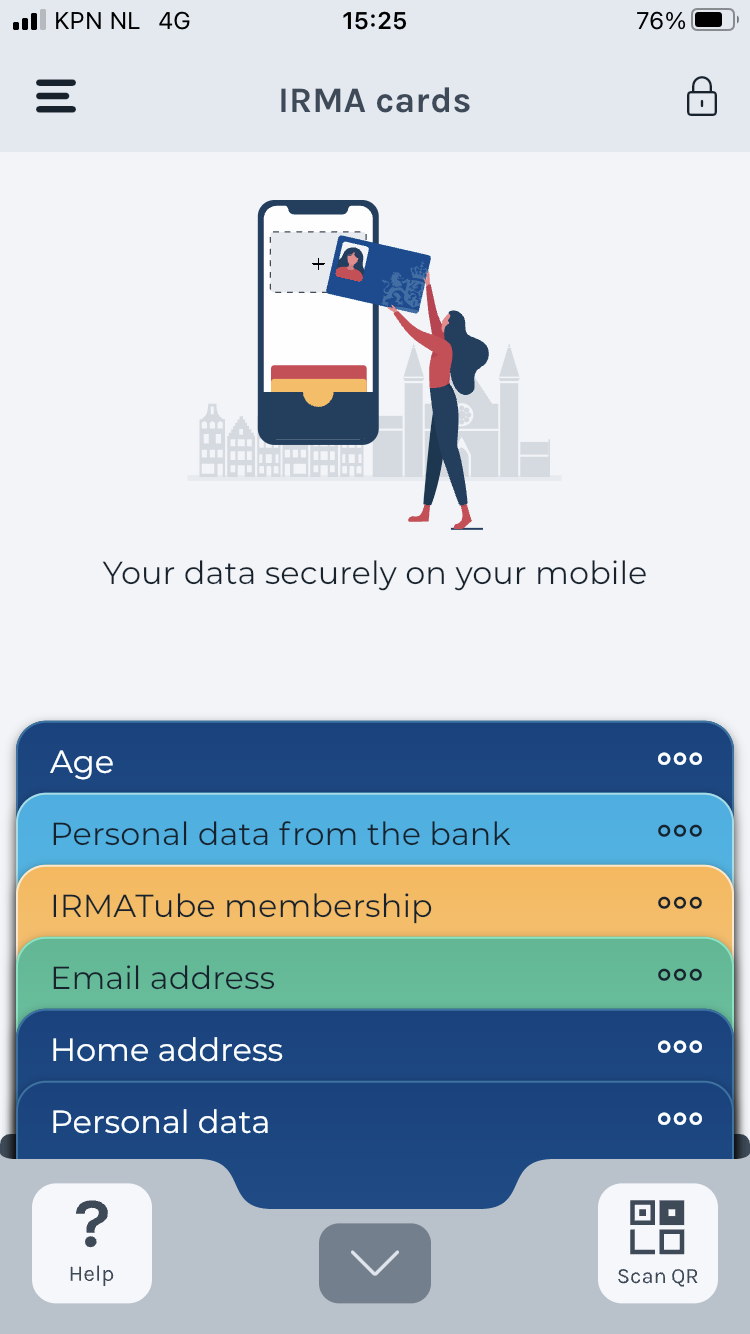
\includegraphics[height=5cm]{Pictures/wallet.png}}
          \only<2->{\begin{minipage}[c][5cm][c]{5.5cm}
            \begin{block}{Email address}
              \vspace{0.5em}
              secret: \textbf{xxxxxxxx}, \\
              Email address: \textbf{\color{blue}maja@irma.app}
              \vspace{0.5em}
            \end{block}
            \begin{tikzpicture}[very thick,overlay, remember picture]
              \draw[red, thick] (5.5,0.5) circle (0.6cm) node {$A, e, v$};
            \end{tikzpicture}
          \end{minipage}}
        \end{center}
      \end{overlayarea}
    \column{0.5\textwidth}
    \begin{center}
      \begin{minipage}[c][3cm][c]{4cm}
        \begin{block}{Diploma}
          \vspace{0.5em}
          secret: \textbf{xxxxxxxx}, \\
          name: \textbf{xxxxxxxx}, \\
          title: \textbf{\only<1>{PhD}\only<2->{{\color{blue}PhD}}}
          \vspace{0.5em}
        \end{block}
        \begin{tikzpicture}[very thick,overlay, remember picture]
          \draw[red, thick] (4,0.5) circle (0.6cm) node {$A, e, v$};
        \end{tikzpicture}
      \end{minipage}
    \end{center}
  \end{columns}
  \note{
    \begin{outline}
      \1 We want to have a wallet, of multiple credentials
      \1 (IRMA app looks is subject to change)
      \1 We need one final step
      \1 It should not be possible for Maja to prove a statement that is not factually true!
      \1 $\Rightarrow$ Solution: in my wallet, we make each credential share the same secret attribute.
      \2 during issuance of a credential to my wallet, we ensure that the credential gets the same secret as that of my other credentials
      \2 During disclosure, prove it to the verifier
      \2 Maja's wallet has a different secret $\Rightarrow$ she can't prove that combination of attributes
    \end{outline}
  }
\end{frame}

\begin{frame}[t]{Idemix - preventing credential pooling attacks}
  \vspace{-0.5cm}
  \begin{columns}[T,onlytextwidth]
    \begin{column}{\textwidth-4cm}
      \begin{center}
        \only<1>{
          \begin{tabular}{rcl}
            $ U = \tilde{A}^{t_e} S^{t_{\tilde{v}}} R_0^{t_0} R_1^{t_1}$ &
            $\xrightarrow{\mathmakebox[3em]{\quad \tilde{A},U\quad}}$ &
          \\[0.5em]
            &
            $\xleftarrow{\mathmakebox[3em]{c}}$ &
            choose random $c$
          \\
            \makecell{$r_e = t_e + ce,\quad r_{\tilde{v}} = t_{\tilde{v}} + c\tilde{v} $\\
            $r_0 = t_0 + ca_0,\quad r_1 = t_1 + ca_1$ } &
            $\xrightarrow{\mathmakebox[3em]{r}}$
            & $U \stackrel{?}{=} \tilde{A}^{r_e} S^{r_{\tilde{v}}} R_0^{r_0} R_1^{r_1}H^{-c}$
          \end{tabular}
        }
        \only<2>{
          \begin{tabular}{rcl}
            $U$ &
            $\xrightarrow{\mathmakebox[3em]{\tilde{A},U}}$ &
          \\[0.5em]
            &
            $\xleftarrow{\mathmakebox[3em]{c}}$ &
            choose random $c$
          \\[0.5em]
            $ r_i = t_i + ca_i $ &
            $\xrightarrow{\mathmakebox[3em]{r_i}}$ &
          \end{tabular}
        }
        \only<3>{
          \begin{tabular}{rcl}
            $ {\color{red}U}, {\color{blue}U}$ &
            $\xrightarrow{\mathmakebox[3em]{{\color{red}\tilde{A}},{\color{red}U}, {\color{blue}\tilde{A}},{\color{blue}U}}}$ &
          \\[0.5em]
            &
            $\xleftarrow{\mathmakebox[3em]{c}}$ &
            choose random $c$
          \\[0.5em]
            $ {\color{red}r_i} = {\color{red}t_i} + c{\color{red}a_i}, \quad {\color{blue}r_i} = {\color{blue}t_i} + c{\color{blue}a_i} $ &
            $\xrightarrow{\mathmakebox[3em]{{\color{red}r_i}, {\color{blue}r_i}}}$ &
          \end{tabular}
        }
      \end{center}
      \uncover<4->{
        Secret key:
        \begin{equation}
          \begin{gathered}
            {\color{red}r_0} = {\color{red}t_0} + c{\color{red}a_0}, \quad {\color{blue}r_0} = {\color{blue}t_0} + c{\color{blue}a_0} \\ \nonumber
            \uncover<5->{\Downarrow \\
            r_0 = t_0 + ca_0}
          \end{gathered}
        \end{equation}%
      }%
      \uncover<5->{%
        User:
        \begin{itemize}
          \item Use same $a_0$ in each credential
          \item When disclosing attributes from multiple credentials, use same $t_0$
        \end{itemize}
        Verifier:
        \begin{itemize}
          \item For each credential, check that the same $r_0$ is used
        \end{itemize}
      }
    \end{column}
    \begin{column}{4cm}
        \begin{flushright}
          \begin{minipage}[c][3cm][c]{3.5cm}
            \begin{block}{Diploma}
              \vspace{0.5em}
              secret: \only<1-2,5>{\textbf{xxxxxxxx}}\only<3-4>{{\color{red}\textbf{xxxxxxxx}}}, \\
              name: \only<1-2>{\textbf{xxxxxxxx}}\only<3->{{\color{red}\textbf{xxxxxxxx}}}, \\
              title: \only<1-2>{\textbf{PhD}}\only<3->{{\color{red}\textbf{PhD}}}
              \vspace{0.5em}
            \end{block}
            \begin{tikzpicture}[very thick,overlay, remember picture]
              \draw[red, thick] (3.5,0.5) circle (0.6cm) node {$\tilde{A}, x, x$};
            \end{tikzpicture}
          \end{minipage}\\
          \uncover<3->{
            \begin{minipage}[c][3cm][c]{3.5cm}
              \begin{block}{Email address}
                \vspace{0.5em}
                secret: \only<1-2,5>{\textbf{xxxxxxxx}}\only<3-4>{{\color{blue}\textbf{xxxxxxxx}}}, \\
                Email address: \\
                \only<1-2>{\textbf{sietse@irma.app}}\only<3->{{\color{blue}\textbf{sietse@irma.app}}}
                \vspace{0.5em}
              \end{block}
              \begin{tikzpicture}[very thick,overlay, remember picture]
                \draw[blue, thick] (3.5,0.5) circle (0.6cm) node {$\tilde{A}, x, x$};
              \end{tikzpicture}
            \end{minipage}
          }
        \end{flushright}
        \vspace{-0.7cm}
        \uncover<5->{
          \centering \hspace{0.5cm}
          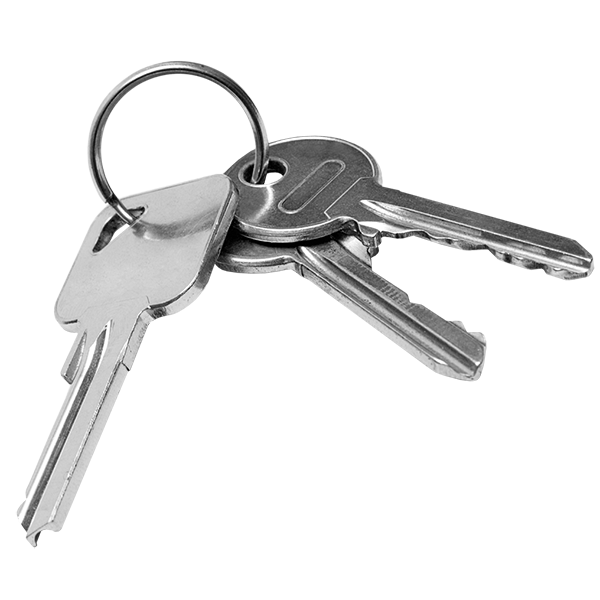
\includegraphics[width=2cm]{Pictures/keyring.png}
        }
    \end{column}
  \end{columns}
\end{frame}

\begin{frame}{Back to the beginning - the total picture}
  \centering
  Self-Sovereign Identity \\[2em]
  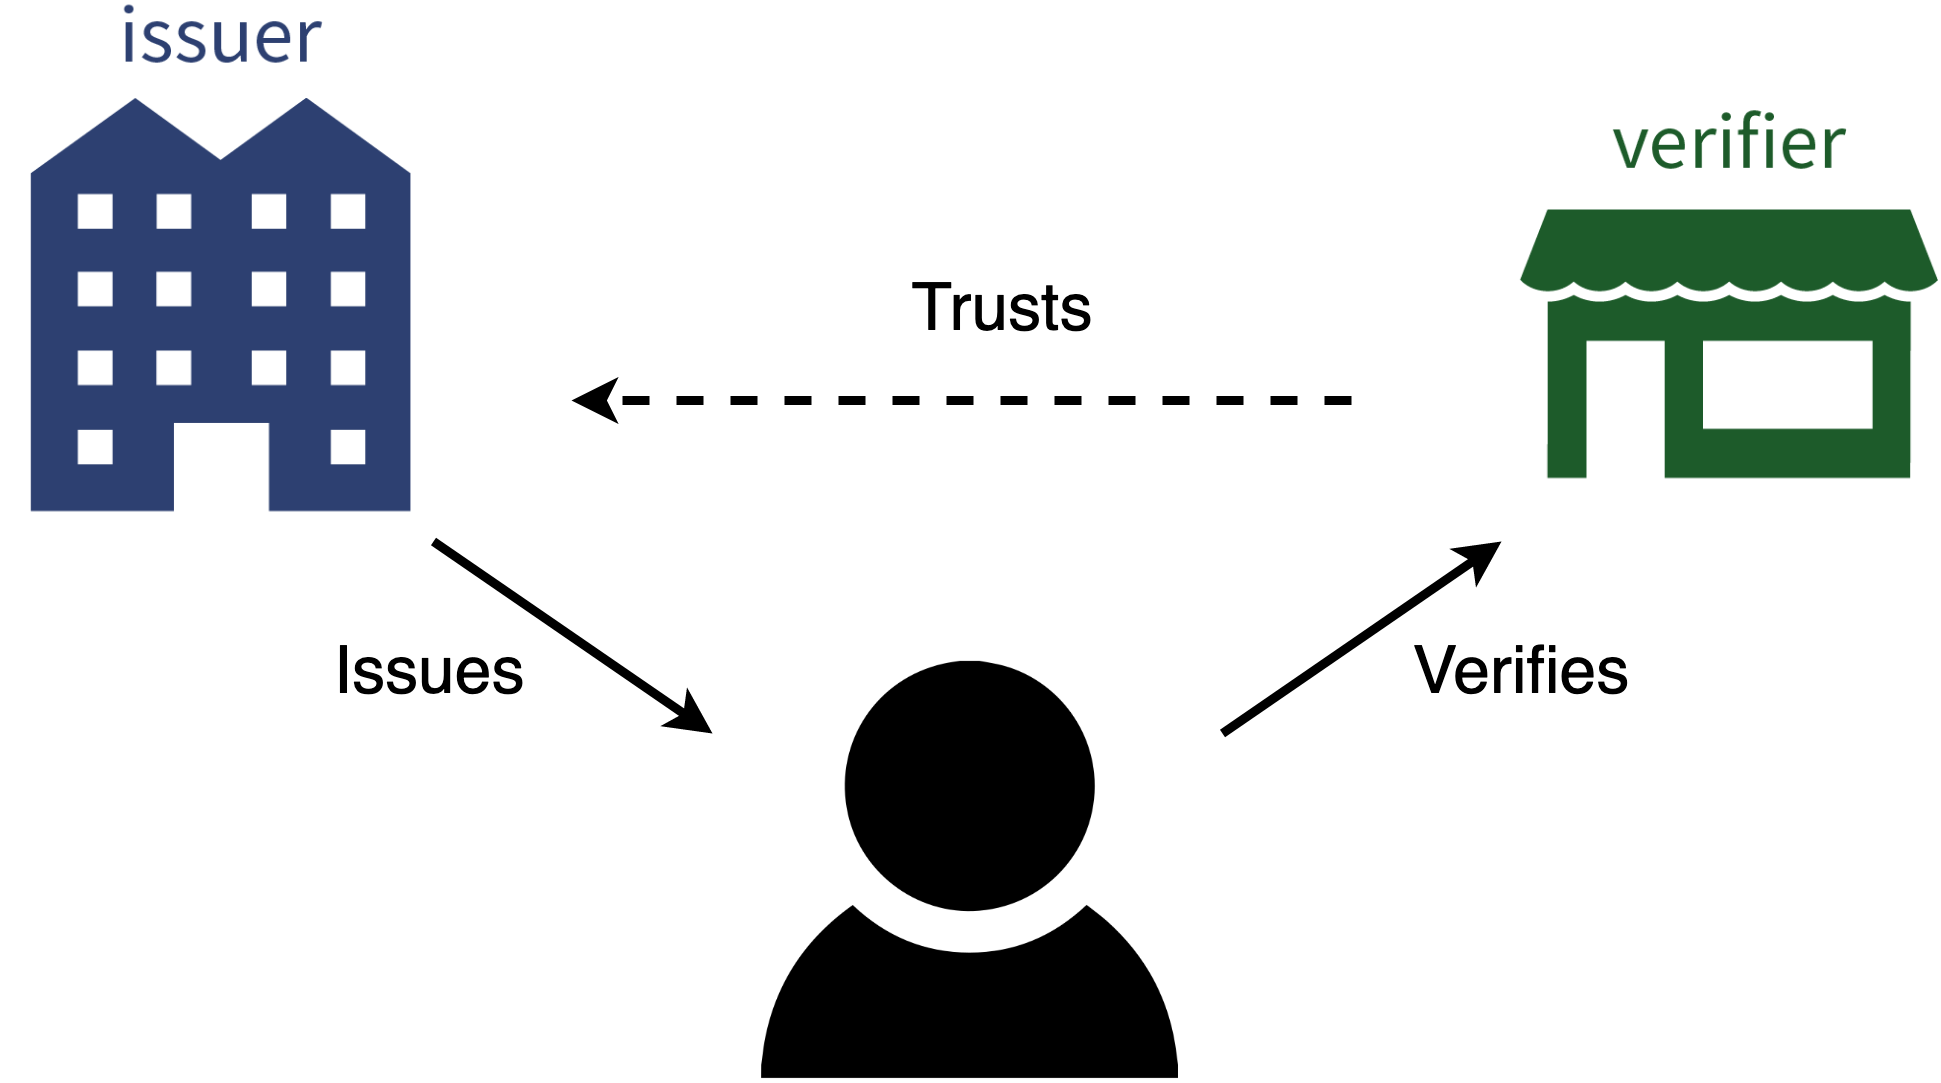
\includegraphics[width=9cm]{Pictures/SSI-diagram.png}
  \note{
    \begin{outline}
      \1 Idemix allows for a wallet of credentials
      \1 You get them from trusted issuers
      \1 You can selectively and unlinkably disclose attributes
      \1 We haven't discussed issuance, or IRMA schemes
      \1 IRMA also has:
        \2 Keyshare server
        \2 Revocation
    \end{outline}
  }
\end{frame}

\begin{frame}[standout]
  The end.
  \note{}
\end{frame}

\begin{frame}{Links}
  \begin{wrapfigure}{r}{0.15\textwidth}
    \centering
    
\includegraphics[width=0.2\textwidth]{Pictures/slideSource.png}
\end{wrapfigure}
Some references:
  \begin{outline}
    \1 Idemix
    \2 IBM Idemix spec: \url{https://dominoweb.draco.res.ibm.com/reports/rz3730_revised.pdf}
    \2 Idemix fact sheet: \url{https://privacybydesign.foundation/pdf/Idemix_overview.pdf}
    \1 Camenisch-Lysyanskaya
    \2 Initial paper: \url{https://www.researchgate.net/profile/Jan-Camenisch/publication/220922101_A_Signature_Scheme_with_Efficient_Protocols/links/5a8c8709458515a4068ae0a3/A-Signature-Scheme-with-Efficient-Protocols.pdf?origin=publication_detail}
    \1 Schnorr protocol
    \2 Initial paper: \url{https://link.springer.com/content/pdf/10.1007/BF00196725.pdf}
    \1 IRMA
    \2 IRMA documentation: \url{https://www.irma.app/docs/what-is-irma/}
    \2 IRMA's Idemix implementation: \url{https://github.com/privacybydesign/gabi/}
   \end{outline}
   %algemene referentie voor credential scheme?
  \note{}
\end{frame}
% if thouroughly annoyed by the alignment, try https://tex.stackexchange.com/questions/160825/modifying-margins-for-one-slide

\begin{frame}[standout]{More slides}
  in case of time or questions
  \note{}
\end{frame}

\begin{frame}{}
  \note{}
\end{frame}

\begin{frame}{Camenisch-Lysyanskaya forgeability if e is constant}
  valid signature 1:$$ Z = A^e S^v R_1^{a_1} \cdots R_{k}^{a_k} $$
  valid signature 2: $$ Z = A'^e S^{\tilde{v}} R_1^{a'_1} \cdots R_{k}^{a'_k} $$
  Combined you get $$ (A/A')^{-e} = S^{v-\tilde{v}} R_1^{a_1-a'_1} \cdots R_{k}^{a_k-a'_k} $$
  This is a valid signature over the attributes $$ a_1-a'_1, ..., a_k-a_k $$
  \note{}
\end{frame}

\begin{frame}{Camenisch-Lysyanskaya's Z to prevent forgeability}
  Formula without Z:\\
  $$ A^e = \frac{1}{S^{v} R_1^{a_1}R_2^{a_2}} \bmod n $$
  \vspace{2em}
  \begin{columns}[onlytextwidth]
    \column{0.5\textwidth}
      \textbf{Example:} Forgery of age attributes.\\
      \vspace{1em}
      $a_1$ ... name (to be hidden)\\
      $a_2$ ... age = 9
      \vspace{1em}
      \column{0.5\textwidth}
      Then I could forge my age to 18, like this:
      claim $a_2 = 18$; \hspace{1em} $a_1' = 2a_1; A' = A^2; v'=2v$
    \end{columns}
  \vspace{1em}
      $$ A'^e = (A^e)^2 = \left(\frac{1}{S^{v} R_1^{a_1}R_2^{a_2}}\right)^2 = \frac{1^2}{S^{2v} R_1^{2a_1}R_2^{2a_2}} = \frac{1}{S^{v'} R_1^{a_1'}R_2^{a_2'}} \bmod n $$
  \note{}
\end{frame}


\begin{frame}{RSA prerequisite on one slide}
  Textbook RSA:\\
  $$A = M^d  \bmod n$$\\
  Verify with: $$A^e = (M^d)^e = M^{de} = M \bmod n$$\\
  \rule{\paperwidth}{0.4pt}\\
  Choose primes p,q and calculate $ n = pq $\\
  Choose e, calculate inverse so that $ e \cdot d = 1 \bmod \phi(n) $ so that $M^{e \cdot d} = M \bmod n$\\
  \rule{\paperwidth}{0.4pt}\\
  Two mathematical hard problems:\\
  1. Discrete logarithm problem: Just knowing A and M it's infeasible to find d.\\
  2. Calculating the inverse of e is hard if you don't know the group order. (It's easy to calculate the group order if you know the prime factorization of n.)
  \note{
    multiplicative group mod n\\
    group order $\phi(n)$ meaning $M^{\phi(n)} = M \bmod n$\\
  }
\end{frame}

\begin{frame}{Keyshare protocol}
  Disclosure session with split secret
  $$\displaystyle \tilde{A}^e = \frac{Z}{S^{\tilde{v}} {\color{red}R_0^{s_k} R_0^{s_u}} R_1^{a_1} R_2^{a_2}} $$
  where the secret $a_0 = s_k s_u$\\
  $s_k$ is only known to the keyshare server\\
  $s_u$ is only known to the app user\\[1em]
  Both $s_k$ and $s_u$ are ALWAYS hidden in Zero Knowledge\\
  To perform the Schnorr protocol with the keyshare server, the app user must provide her PIN
  \note{}
\end{frame}

\begin{frame}[plain]
  \vspace{-0.3cm}
    \begin{figure}
    \[
    \begin{array}{c c c c c}
    \textbf{TTP} & & \textbf{User} & & \textbf{Issuer}\\
    N, R; m_t & & N, R; m_u, P_t & \XLR{\text{Issuance}} & N, R \\
     & & \text{Choose random } w_u & \XL{\text{nonce }\eta} & \\
     & & W_u = R^{w_u} \bmod N & & \\
     \text{Choose random } w_t & \XL{P_u, h_W} & h_W = \mathcal{H}(W_u) & & \\
    W_t = R^{w_t} \bmod N & \XR{W_t} & W = W_uW_t & & \\
     & & c = \mathcal{H}\left(\eta, P, W\right) & & \\
    \text{verify } h_W = \mathcal{H}(W_u) & \XL{\eta, c, s_u, W_u} & s_u = w_u + cm_u & & \\
    \text{verify }R^{s_u} = P_u^cW_u \bmod N & & & & \\
    P = P_uP_t,\, W = W_uW_t & & & & \\
    \text{verify }c = \mathcal{H}(\eta, P, W) & & & & \\
    s_t = w_t + cm_t & & & & \\
    s = s_u + s_t & & & & \\
    \sigma = \text{sign}\left(\text{sk}, \left(c,s\right)\right) & \XR{\sigma, s} & & \XR{\sigma, c, s, P} &  \text{verify}\left(\text{pk}, \sigma, \left(c,s\right)\right)\\
     & & & & W = R^sP^{-c} \bmod N \\
     \text{\color{red}{[Figure credits: see notes]}}& & & & \text{verify }c = \mathcal{H}\left(\eta, P, W\right)
    \end{array}
    \]
    \end{figure}
  \note{
    \begin{itemize}
      \item Very ugly, detailed version of the keyshare server protocol.
      \item Just in case there are questions.
      \item Figure adjusted from "A provably secure keyshare protocol" by David Venhoek and Sietse Ringers
    \end{itemize}
  }
\end{frame}

\begin{frame}{Revocation of credentials - Issuance}
  The current accumulator is a number $\nu \in QR_n$. The first accumulator is randomly chosen by the issuer from $QR_n$. During issuance, the issuer\\

  \begin{enumerate}
    \item generates a prime $e$,
    \item embeds the prime $e$ as an attribute within the credential being issued,
    \item uses its private key to compute $u = \nu^{1/e\bmod pq}$, and sends the tuple $(u,e)$ to the app along with the credential,
    \item stores the number $e$ in a database for later revocation.
  \end{enumerate}

\end{frame}

\begin{frame}{Revocation of credentials - Disclosure}
  The revocation witness is the tuple $(u, e)$. By definition it is valid only if $u^e = \nu \bmod n$. When using revocation, the app now proves the following to the verifier:\\
  \begin{itemize}
    \item "I possess a valid credential containing the disclosed attributes as well as an undisclosed attribute $e$."
    \item "I know a number $u$ which is such that $u^e = \nu \bmod n$."
  \end{itemize}
\end{frame}

\begin{frame}{Revocation of credentials - Revocation}
  Compute new accumulator value:
  $$\displaystyle \nu_{i+1} = \nu_{i}^{1/\tilde{e}\bmod pq}$$
  Update witness:
  $$\displaystyle u_{i+1} = u_i^b\nu_{i+1}^a$$
  Proof that update mechanism works:
  $$
  u_{i+1}^{e} = (u_i^b\nu_{i+1}^a)^{e}
  = u_i^{be}\nu_{i+1}^{ae} 
  = \nu_i^{b}\nu_{i}^{ae/\tilde{e}}
  = (\nu_i^{b\tilde{e}}\nu_{i}^{ae})^{1/\tilde{e}}
  = (\nu_i^{b\tilde{e}+ae})^{1/\tilde{e}} 
  = \nu_i^{1/\tilde{e}}
  = \nu_{i+1}
  $$
  \note{
    % https://www.irma.app/docs/revocation/#cryptography
    % "Accumulators with applications to anonymity-preserving revocation" (https://eprint.iacr.org/2017/043.pdf)
    % which is based on "Dynamic accumulators and application to efficient revocation of anonymous credentials" (http://static.cs.brown.edu/people/alysyans/papers/camlys02.pdf)
    }
\end{frame}

% \begin{frame}{Becoming part of the community}
%   links naar repo's en slack
%   \note{}
% \end{frame}

% \begin{frame}{Range proofs}
%   \note{}
% \end{frame}

% \begin{frame}{Number sizes}
  % bit lengths of S (and hence, Z, R's, A), pq, a, e, v
  % bit lengths of random t,c from Schnorr
  % bit lengths of random r from unlinkability
%   \note{}
% \end{frame}

% \begin{frame}{An example with numbers only}
%   \note{}
% \end{frame}

% \begin{frame}{A word on blockchain}
%   \note{}
% \end{frame}

% \begin{frame}{Other credential schemes}
%   WIP
  % \begin{tabular}{l|l|l|l|l|l|l|l|l}
  %   scheme & efficiency & hardness & type & PQ* safe & \makecell{prov\\able} & \makecell{unforge\\able} & \makecell{unlink\\able} & SD*\\
  %   \hline
  %   CL* &  & \makecell{strong RSA\\assumption} & RSA & \cellcolor{red} & \cellcolor{green} & \cellcolor{green} & \cellcolor{green} & \cellcolor{green} \\
  %   \hline
  %   certificates &&&&&&&& \\
  %   \hline
  %   Schnorr &&&&&&&& \\
  %   \hline
  %   Fiat-Shamir &&&&&&&& \\
  %   \hline
  %   \makecell{Gennaro, Halevi,\\ Rabin} &&&&&&&& \\
  %   \hline
  %   Cramer, Shoup &&&&&&&& \\
  %   \hline
  %   UProof &&&&&&&& 
  %   % other ABC that are newer??\\
  % \end{tabular}

  % *CL = Camenisch-Lysyanskaya\\
  % PQ = post-quantum\\
  % SD = selective disclosure
  % \note{
    % provability is a must if you want to actually use the system. exception for UProof's unlinkability proof (why?)
  % }
% \end{frame}

% Misschien
%   QR
%   keyshare
%   revocation
%   range proofs

% Achtergrond
%   verschillen tussen IRMA en vanilla Idemix
%   andere ABCs (U-Prove, BBS+, RVH)

\end{document}

MCH Idemix IRMA crypto praatje

inleiding
  standaardplaatje
  signature schemes
  credential schemes (bv x509 cert)
    RSA toy credential scheme
    probleem: niet selective, linkable

Opbouw
  signature scheme
  selective disclosure, gratis challenge-response
  unlinkability
  meerdere credentials disclosen

CL sig scheme
  Begin bij RSA: A^e = M mod n
  vervang M met M = \frac{bla}{bla}
  e is variabel, (A,e,v)
  strong RSA assumption
Selective disclosure
  middels ZKP
  https://latexpad.clrnd.com.ar/#f78aa65b4a4d1918f10a2e9210906507, standaard 3-move diagram
  evt: 1 attribuut -> meerdere attributen tegelijk
  ? fiat-shamir
  ? niet commitment maar challenge opsturen
Unlinkability
  A omvormen: A -> AS^r,  v -> v - er
  (e, v) verbergen
combinatie van dit alles: selective unlinkable disclosure (met één issuer)
  disclosure protocol laten zien
Idemix: meerdere issuers
  voorkomen: Maja Reißner, PhD
  attribuut 0: random secret key, hetzelfde in alle credentials
  tijdens disclosure: bewijzen dat attr 0 uit alle credentials hetzelfde is
-> standaardplaatje

Als het past
  relatie met gabi

Misschien
  QR
  keyshare
  revocation
  range proofs

Achtergrond
  verschillen tussen IRMA en vanilla Idemix
  andere ABCs (U-Prove, BBS+, RVH)
